% !TEX root=/home/tavant/these/manuscript/src/manuscript.tex

\section{ Discussion on the radial wavenumber}
  \label{sec-DR-BC}
    
  In the \ac{ECDI} dispersion relation described in \cref{sec-DR-kinetic}, the radial wavenumber must be non-zero.
  Hence, in \cref{sec-DR-results}, we have chosen a wavelength that fits between the two walls.
  On the other hand, the oscillation seen in \cref{fig-phi_fluctuation_summary} seems not to present any oscillation in the radial direction.
  In this section, we investigate the interaction between the azimuthal instability and the wall in the radial direction.
  
  \subsection{Radial profile of the oscillation} \label{subsec-radial_prof}
  \Cref{fig-phi_osci_profile} shows the amplitude of the azimuthal instability on the plasma potential.
  It is defined as
  \begin{equation} \label{eq-stdphi}
    \delta \phi^2 = 2 \sigma_{\phi}^2 = \frac{{2}}{L_{\theta}} \int_0^{L_{\theta}} \lp  \phi - <\phi>_{\theta}  \rp ^2 d\theta,
  \end{equation}
  
  \begin{figure}[hbt]
    \centering
    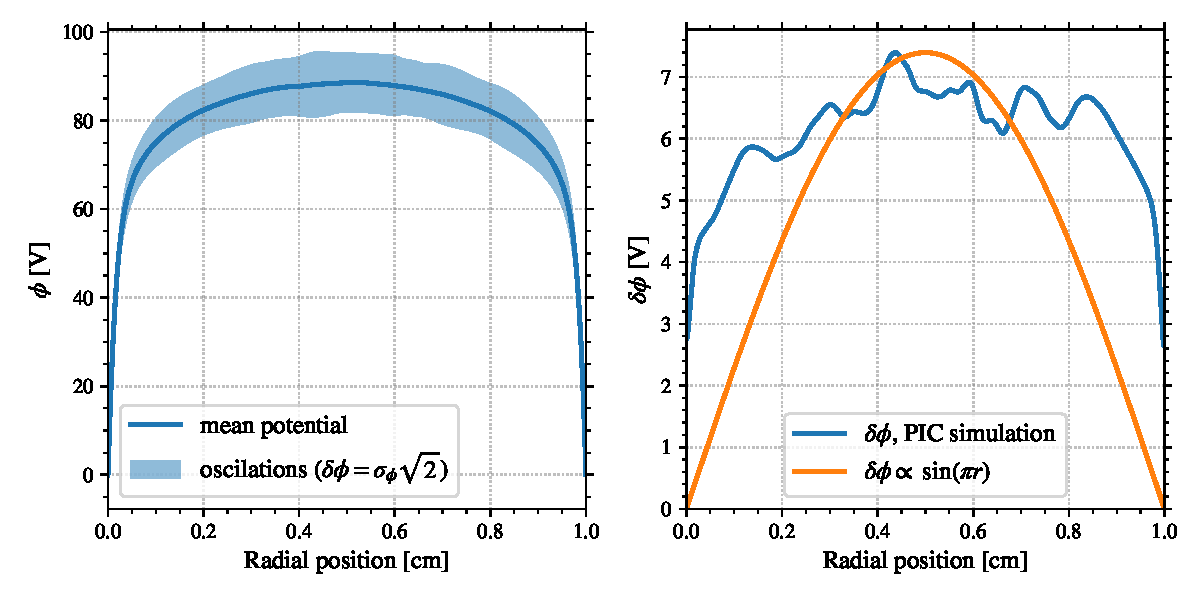
\includegraphics[width=\textwidth]{phi_oscillation}
    \caption{(Left) Radial profile of the mean plasma potential averaged in the azimuthal direction  and in time during the steady-state of the simulation ($t > 3.5 \,\micro\second$) and the average azimuthal instability amplitude. (Right) Radial profile of the  azimuthal instability amplitude, compared with a sinusoidal profile. }
    \label{fig-phi_osci_profile}
  \end{figure}
  
  
  We see in \cref{fig-phi_osci_profile} that the amplitude of the oscillation in the radial direction does not follow a sinusoidal profile, that would be the characteristic of a non-zero radial wavenumber.
  This observation contradicts the hypothesis made previously on the value of $k_r$.
  In order to better apprehend the radial profile of the instability amplitude, we study the ratio between $\delta \phi$ the fluctuation amplitude (showed on the right in \cref{fig-phi_osci_profile}) and $<\phi>_{\theta}$  the mean plasma potential (on the left in \cref{fig-phi_osci_profile}).
  
  \begin{figure}[hbt]
    \centering
    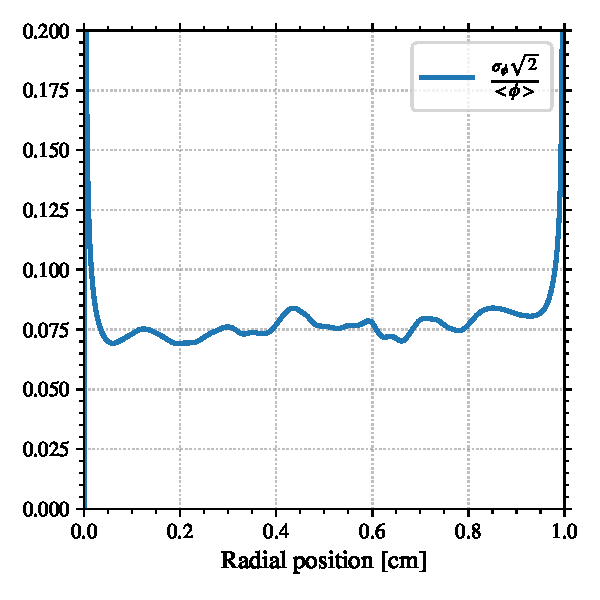
\includegraphics[width=\defaultwidth]{phi_oscillation_ratio}
    \caption{Radial profile of the ratio between $\delta \phi$ the fluctuation amplitude (showed on the right in \cref{fig-phi_osci_profile}) and $<\phi>_{\theta}$  the mean plasma potential (on the left in \cref{fig-phi_osci_profile}).}
    \label{fig-ratio}
  \end{figure}
  
  \Cref{fig-ratio} shows that the ration $\frac{\delta \phi}{ <\phi>_{\theta}}$ is almost constant in the plasma, except close to the wall, where the plasma potential decreases much faster than the oscillations.
  The same behavior  observed in the profiles of the ion density, that can be seen in \Cref{fig-ion_oscilation}.
  As a mater of fact, the behavior even more pronounced on the ion density, as the ratio $\delta n_i / n_i$ presents a radial profile almost constant.
  It can be explains by the fact the ions reaches the wall with an supersonic speed, so that the wall does not directly affected the ions.
  
  
  \begin{figure}[hbt]
    \centering
    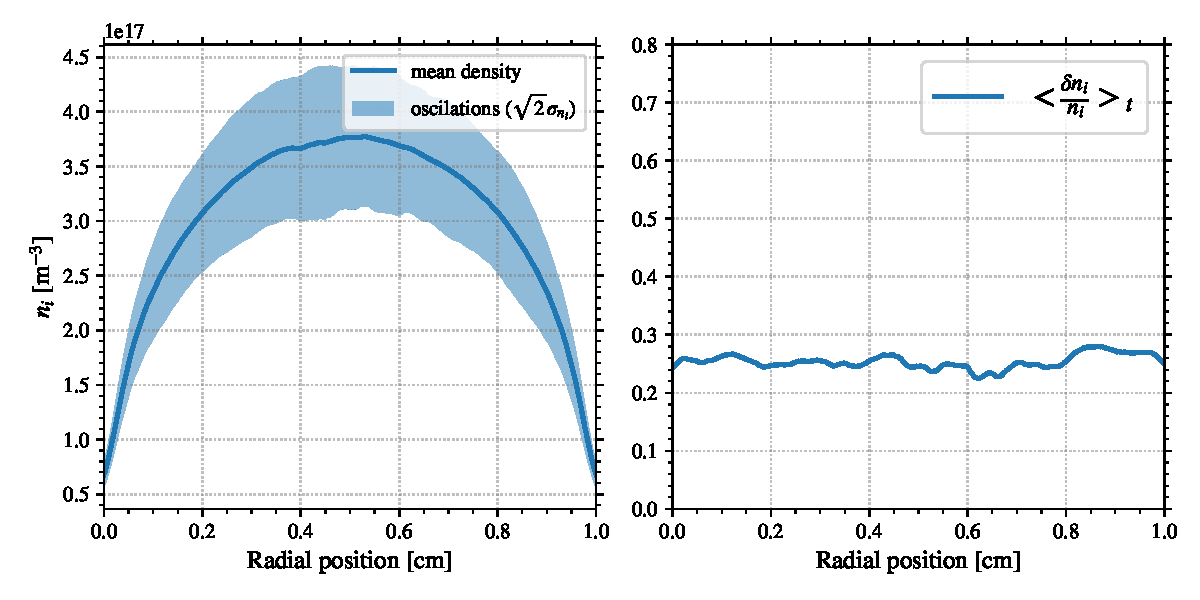
\includegraphics[width=\textwidth]{Ion_oscilations.pdf}
    \caption{Radial profile of (left) the mean ion density profile and $\delta n_i$ the fluctuation amplitude and (right) the ratio between $\delta n_i$ and $n_i$.}
    \label{fig-ion_oscilation}
  \end{figure}
  
  \vspace{1em}
  This may suggest that the sheaths screen  the walls significantly from the oscillations,  which are therefore not affected.
  A screening of the wall have been observed in \citet{janhunen2018}, where the authors observed radial structures of wavelength larger than the radial length.
  However, here we observe no radial structure.
  The difference between  \citet{janhunen2018} and the results presented here may be due to the difference in the radial length ($L_R =1 \,\centi\meter$ here, against $L_R = 5.38\,\centi\meter$).
  
  \subsection{Impact of the radial wavenumber on the \ac{DR}}
   \label{subsec-kr}

  To highlight the impact of the radial wavenumber on the \ac{ECDI} \ac{DR}, \cref{fig-kreffect} shows for three values of $k_r \lde$ the evolution of the frequency $\omega$, and  the growth rate $\gamma$ as a function of the azimuthal wavenumber $k_{\theta}$.
  We see that when $k_r \lde$ increases from 0.02 to 0.1, the cyclotron resonances decrease and broaden until they disappear.
  \begin{figure}[!hbt]
    \centering
    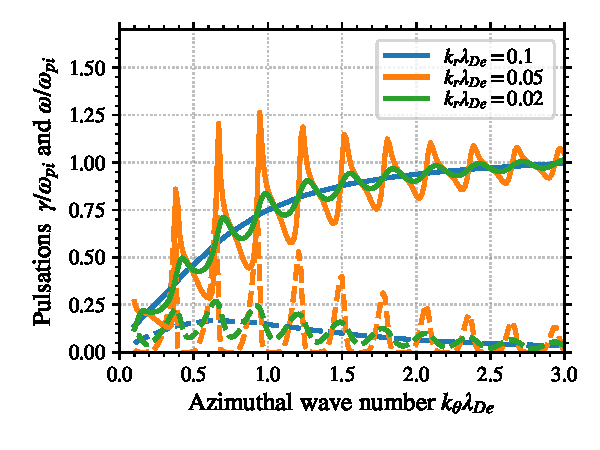
\includegraphics[width=\defaultwidth]{ECDI_ktheta_impact.pdf}
    \caption{Evolution as a function of the azimuthal wavenumber $k_{\theta}$ of (solid line) the frequency $\omega$, and (dashed line) the growth rate $\gamma$ for three values of the normalized radial wavenumber $k_r \lde$. }
    \label{fig-kreffect}
  \end{figure}
  
  This reduction of the resonances explains the observations of \cref{fig-DRECDI}, where we saw similar reduction of the cyclotron resonances, due to the increase of $\lde$ the Debye length from $\lde=\sn{4.3}{-5}\,\meter$ at $t=0$ to $\lde=\sn{7.0}{-5}\,\meter$ at saturation.
  However, if the radial wavenumber $k_r$ tends toward zero, in agreement with the observations of \cref{fig-ion_oscilation}, then the resonances would not smooth out for this reason.
  Instead, the resonances would stay.
  
  \vspace{1em}
  As a conclusion, the interaction between the instability and the boundaries is not clearly understood.
  The sheaths seem to  screen the waves from the radial boundaries.
  In \Cref{subsec-BC}, we will discuss on the impact of the radial boundary condition (metallic versus dielectric electrode) on the oscillation, but the conclusion will be similar.

  As there is no radial structure observed in the simulation showed here, it means that the oscillation is purely azimuthal, or at least $\lde k_r <<1$.
  In this case, the cyclotron resonances should non-longer disappear \citep{ducrocq2006}, except due to non-linear demagnetization of the electrons, as discussed before \citep{boeuf2018,taccogna2019}.
  The non-linear dispersion relations are out of the scope of the present work, but should be developed in order to better understand the evolution on the \ac{ECDI} in the \ac{HET}.
  
  To understand the divergent observations of \citet{hara2019a,janhunen2018,taccogna2019}, a comparisons of the simulation results using similar parameter and models should be undertaken.
  Such a comparison is currently undertook between the different working groups on another simulation case. 
  Once this first Benchmark is conducted, the radial-azimuthal geometry should be studied.
  
  
  
  